%% 
%% Copyright 2007-2024 Elsevier Ltd
%% 
%% This file is part of the 'Elsarticle Bundle'.
%% ---------------------------------------------
%% 
%% It may be distributed under the conditions of the LaTeX Project Public
%% License, either version 1.3 of this license or (at your option) any
%% later version.  The latest version of this license is in
%%    http://www.latex-project.org/lppl.txt
%% and version 1.3 or later is part of all distributions of LaTeX
%% version 1999/12/01 or later.
%% 
%% The list of all files belonging to the 'Elsarticle Bundle' is
%% given in the file `manifest.txt'.
%% 
%% Template article for Elsevier's document class `elsarticle'
%% with numbered style bibliographic references
%% SP 2008/03/01
%% $Id: elsarticle-template-num.tex 249 2024-04-06 10:51:24Z rishi $
%%




\documentclass[preprint,12pt]{elsarticle}
\usepackage{graphicx} % Required for inserting images
\usepackage{amsmath,amssymb,amsfonts}
\usepackage{physics}
\usepackage{ae}
\usepackage{epsfig}
\usepackage{amsmath}
\usepackage{amssymb}
%\usepackage{subfig}
\usepackage{multirow}
\usepackage{amsthm}
\usepackage{url}         % formats URL addresses properly
\usepackage[title]{appendix}%    % allows appendix section to be included
\usepackage{lscape}      % allows a page to be rendered in landscape mode
\usepackage{multicol}    % allows text in multi columns
\usepackage{cancel}      % needed to show canceled terms in equations
\usepackage{lettrine}
\usepackage{placeins}
%my packages
\usepackage{comment}
\usepackage{array}
\usepackage{adjustbox}
\usepackage{wrapfig}
\usepackage[table]{xcolor}
\usepackage{amsmath}
\usepackage[most]{tcolorbox}
\usepackage{tikz}
\usepackage{pgfplots}
\usepackage{amsfonts} 
\usepackage{float}
\usepackage{subcaption}
\usepackage[labelsep=space]{caption}
\usepackage{algpseudocode}
\usepackage{algorithm}
\usepackage{algorithmicx}%
\usepackage{diagbox}
\usepackage{lipsum}
\usepackage{textcomp}
\usepackage{listings}
\usepackage{circledsteps}
\usepackage{mathrsfs}%
\usepackage{manyfoot}%
\usepackage{booktabs}%
\usepackage{hhline, multirow}
\usepackage{tabulary}
\usepackage{enumitem}
\usepackage{slashbox}
\usepackage{nicematrix}
\usepackage{circledsteps}
\usepackage{physics}
\usepackage{pifont} % xmark

\urldef\myurl\url{https://research.cec.sc.edu/files/cyberinfra/files/5-%20Setting%20WAN%20Bandwidth%20with%20Token%20Bucket%20Filter%20%28TBF%29.pdf}

\urldef\sysctlurl\url{https://research.cec.sc.edu/files/cyberinfra/files/Lab%206.pdf}

%%
%%Abreviaturas
%%%%%Deep Learning Neural Networks (DLNN)
%%%%%Congestion Control (CC)
%%%Recurrent Neural Networks (RNN)




%\title{UAT}
%\author{crereis }
%\date{July 2025}




\newcommand{\dirfig}{%
	%~/Doutorado/figuras
	%./figs%
}

\newcommand{\dirfigs}{%
	%\dirfig
}

\newcommand{\fnbridgewifi}{%
\footnote{\url{https://ueevii.com/products/ueevii-cpe450-100mbps-3km-point-to-point-wireless-bridge-2-pack}}%
}

\newcommand{\fnsatelite}{%
\footnote{\url{https://www.starlink.com/br/business}}%
}

\newcommand{\fnfso}{%
\footnote{\begin{tabular}[c]{@{}c@{}}\\ \url{https://www.nasa.gov/technology/6-things-you-need-to-know-about-nasas-laser-communications}\\ \url{-relay-demonstration/}\end{tabular}}%
}


\newcommand{\fnqm}{%
\footnote{The QM starts a record every five nanoseconds, but this process, even if in a mapped-memory file, could take more than that. So, the timestamps in the QM column in Table \ref{tab:bmf_generating} do not differ by five nanoseconds.}%
}

\newcommand{\cc}[1]{\cellcolor{lightgray}#1} %cc -> collor cell

\newcommand{\mr}[1]{
	\multirow{2}{3em}{#1}%
}
\newcommand{\fontsdir}{%
	./fonts%
}


\newcommand{\fncolab}{%
	\footnote{\url{https://colab.google/}}%
}


\newcommand{\fnfsoerror}{%
	\footnote{\url{https://support.transcelestial.com/support/solutions/articles/51000324695-bit-error-rates-what-is-ber-and-what-is-a-good-ber-}}
}

\newcommand{\fnc}{%
\footnote{Every time the article mentions \textit{``the previous work''}, it refers to the Marcondes and Silva article referenced by \cite{b0000078}, which is a short version of this paper, utilizing just one bottleneck rate (10Mbps), up to 40 flows, and based on a simulated environment.}%
}%

\newcommand{\fnbbr}{\footnote{https://cloud.google.com/blog/products/networking/tcp-bbr-congestion-control-comes-to-gcp-your-internet-just-got-faster}}


\newcommand{\fntcpdumplibpcap}{%	
	\footnote{\url{https://www.tcpdump.org/}}%
}

\newcommand{\fnsysctlcongcontrol}{%	
	%\footnote{\url{https://research.cec.sc.edu/files/cyberinfra/files/Lab\%206.pdf}}%
	\footnote{\sysctlurl}%
}

\newcommand{\fnnetem}{%	
	\footnote{\url{https://man7.org/linux/man-pages/man8/tc-netem.8.html}}%
}


\newcommand{\fnwestwoodwinsbbr}{\footnote{Among the traditional variants, BBR presented the highest normalized throughput in  practically all tests, losing by a very close (0.007) margin to WestwoodPlus in a single round, with 80 flows at 10Mbps.}}

\newcommand{\fnfontbbr}{%
	\footnote{\url{https://git.kernel.org/pub/scm/linux/kernel/git/stable/linux.git/tree/net/ipv4/tcp_bbr.c?h=v6.15.2}} %
}

\newcommand{\model}[2]{%
	#1$_{#2}$%
}


%

\renewcommand{\figurename}{Fig.}


\newcommand{\xmark}{\ding{55}}


\newcommand{\fnnotebooks}{\footnote{For each bottleneck, the research data (training, generalization, and iPerf throughput) and notebooks used during experiments are available at https://drive.google.com/file/d/1gZvA2ut1TKcIkmOjJpN3O1ZNiUI08Cvo/view?usp=sharing.}}









%% Use the option review to obtain double line spacing
%% \documentclass[authoryear,preprint,review,12pt]{elsarticle}

%% Use the options 1p,twocolumn; 3p; 3p,twocolumn; 5p; or 5p,twocolumn
%% for a journal layout:
%% \documentclass[final,1p,times]{elsarticle}
%% \documentclass[final,1p,times,twocolumn]{elsarticle}
%% \documentclass[final,3p,times]{elsarticle}
%% \documentclass[final,3p,times,twocolumn]{elsarticle}
%% \documentclass[final,5p,times]{elsarticle}
%% \documentclass[final,5p,times,twocolumn]{elsarticle}

%% For including figures, graphicx.sty has been loaded in
%% elsarticle.cls. If you prefer to use the old commands
%% please give \usepackage{epsfig}

%% The amssymb package provides various useful mathematical symbols
\usepackage{amssymb}
%% The amsmath package provides various useful equation environments.
\usepackage{amsmath}
%% The amsthm package provides extended theorem environments
%% \usepackage{amsthm}

%% The lineno packages adds line numbers. Start line numbering with
%% \begin{linenumbers}, end it with \end{linenumbers}. Or switch it on
%% for the whole article with \linenumbers.
%% \usepackage{lineno}

\journal{Ad Hoc Networks}

\begin{document}

\begin{frontmatter}

%% Title, authors and addresses

%% use the tnoteref command within \title for footnotes;
%% use the tnotetext command for theassociated footnote;
%% use the fnref command within \author or \affiliation for footnotes;
%% use the fntext command for theassociated footnote;
%% use the corref command within \author for corresponding author footnotes;
%% use the cortext command for theassociated footnote;
%% use the ead command for the email address,
%% and the form \ead[url] for the home page:
%% \title{Title\tnoteref{label1}}
%% \tnotetext[label1]{}
%% \author{Name\corref{cor1}\fnref{label2}}
%% \ead{email address}
%% \ead[url]{home page}
%% \fntext[label2]{}
%% \cortext[cor1]{}
%% \affiliation{organization={},
%%             addressline={},
%%             city={},
%%             postcode={},
%%             state={},
%%             country={}}
%% \fntext[label3]{}

\title{Deep Learning-Prompted TCP Congestion Control to Explore High-Error Link Transmission Potential.}



%% use optional labels to link authors explicitly to addresses:
%% \author[label1,label2]{}
%% \affiliation[label1]{organization={},
%%             addressline={},
%%             city={},
%%             postcode={},
%%             state={},
%%             country={}}
%%
%% \affiliation[label2]{organization={},
%%             addressline={},
%%             city={},
%%             postcode={},
%%             state={},
%%             country={}}


%% Author affiliation

\begin{comment}


\affiliation[ita]{organization={Department of Electronics and Computer Engineering - Aeronautics Institute of Technology (ITA)},%Department and Organization
	addressline={Praça Marechal Eduardo Gomes}, 
	city={São José dos Campos},
	postcode={12228-900}, 
	state={SP},
	country={Brasil}}

\cortext[cor1]{crereis@gmail.com}

\fntext[oead]{cesar.marcondes@gp.ita.br}


\author[ita]{Marcelo Silva\corref{cor1}} %% Author name
\author[ita]{Cesar Marcondes\fnref{oead}}
\end{comment}


%% Abstract

%%Graphical abstract


\end{frontmatter}

%% Add \usepackage{lineno} before \begin{document} and uncomment 
%% following line to enable line numbers
%% \linenumbers

%% main text
%%

%\section{Data Mining} \label{sec:data_mining}
\newcommand{\fngitrouterconfigscript}{%
	\footnote{The RT configuration script for setting IP routes, speed, and RTT of the connections is available in  \url{https://github.com/reisdout/git-udt/blob/main/scripts/config_router.sh}}%
}

\vspace{-3cm}

\begin{figure}[h!t]
	\centering
	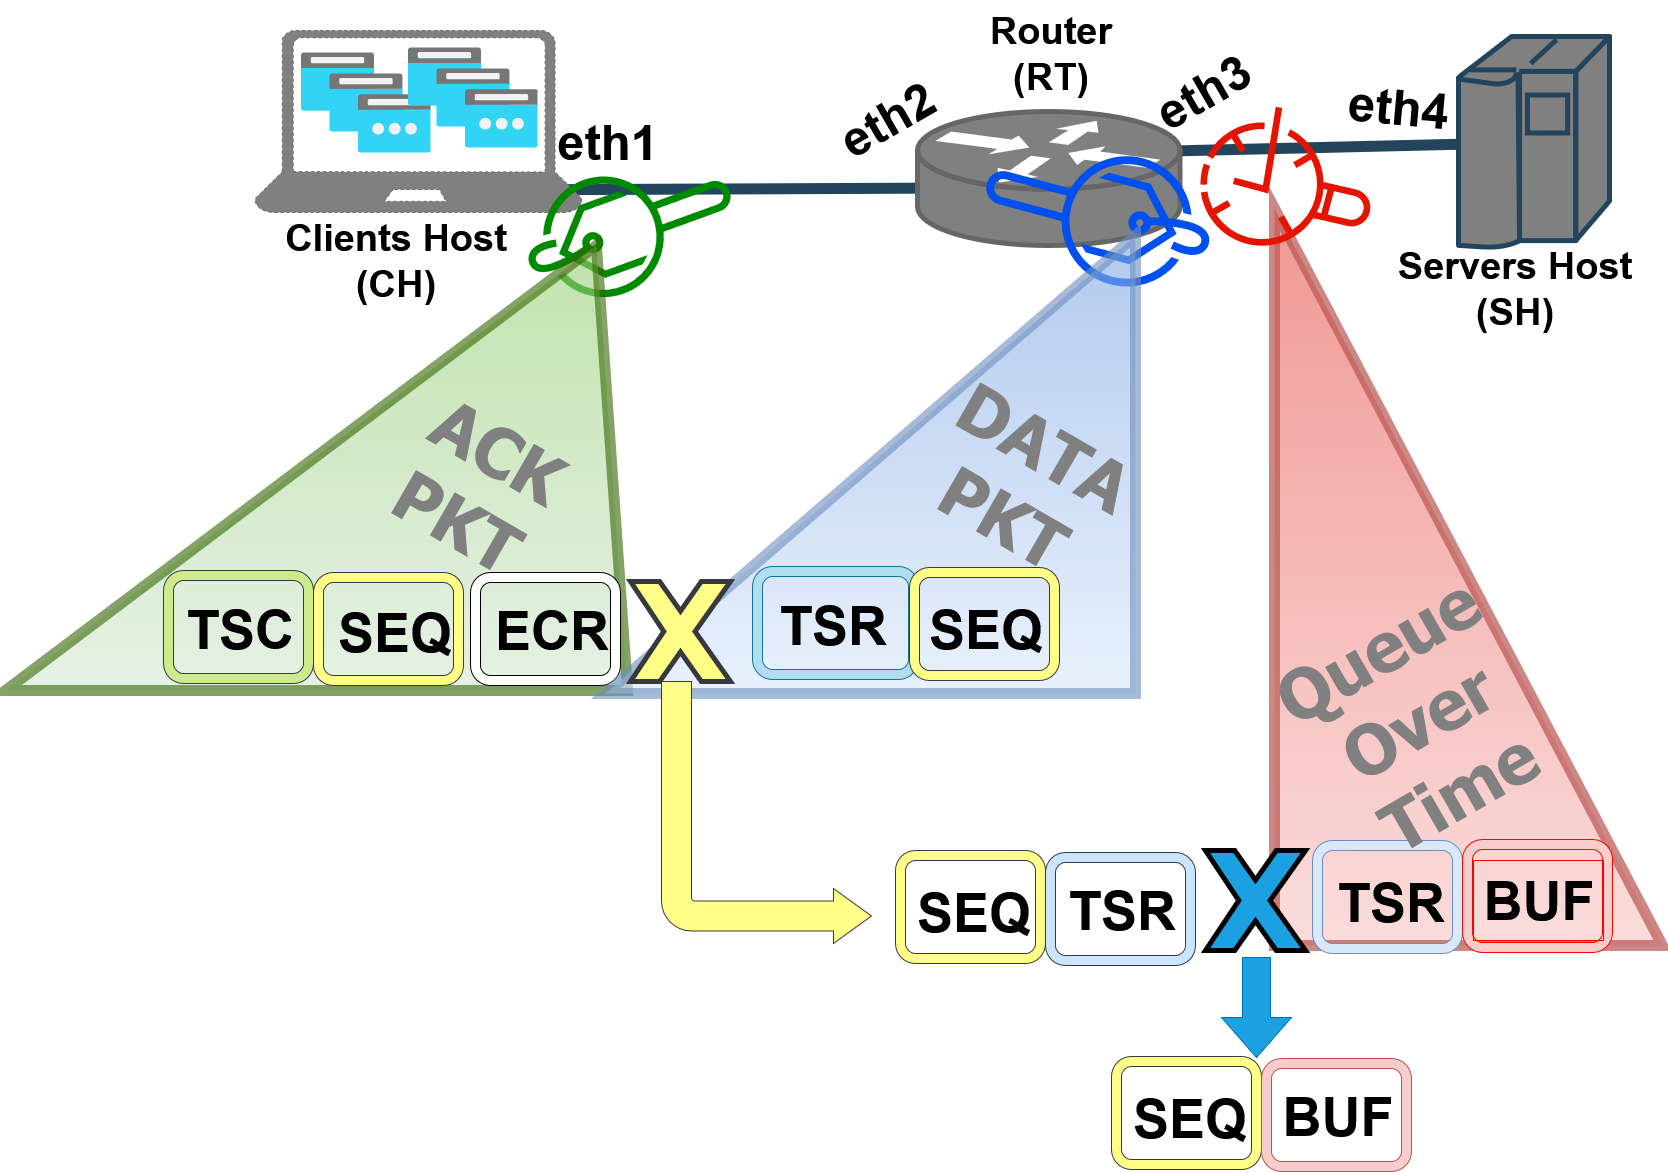
\includegraphics[width=0.6\textwidth]{figure_0006.png}
	%\caption{}
	\label{fig:dumbell_poc}
\end{figure}    


\begin{table}[h]
	\centering
	\caption{Configuration of PoC setup machines.}
	%\centering
	\begin{tabular}{|c|m{0.9\linewidth}|}		\hline
		Machine & \hspace{0.4\linewidth}Spec \\ \hline
		Clients Host (CH) & \textbf{OS}: Linux Mint 22 x86\_64; \textbf{Kernel}: 6.8.0-38-generic; \textbf{CPU}: 12th Gen Intel i7-12700H (20) @ 4.600GHz; \textbf{Memory}: 3050MiB / 64052MiB; \textbf{Ethernet interface}: RTL8125 2.5GbE Controller -vendor: Realtek Semiconductor Co., Ltd. \\
		& \\
		Router (RT) & \textbf{OS}: Linux Mint 22 x86\_64; \textbf{Kernel}: 6.8.0-52-generic; \textbf{CPU}: Intel Atom C2758 (8) @ 2.400GHz; \textbf{Memory}: 1015MiB / 7912MiB; \textbf{Ethernet interface}: Ethernet Connection I354 - vendor: Intel Corporation \\
		&\\
		Servers Host (SH) & \textbf{OS}: Linux Mint 22 x86\_64; \textbf{Kernel}: 6.8.0-38-generic; \textbf{CPU}: 11th Gen Intel i7-1165G7 (8) @; \textbf{Memory}: 1347MiB / 15790MiB; \textbf{Ethernet interface}: RTL8111/8168/8211/8411 PCI Express Gigabit Ethernet Controller - vendor: Realtek Semiconductor Co., Ltd. \\ \hline
	\end{tabular}	
	\label{tab:poc_setup_machines_spec}
\end{table}




\begin{comment}

%% Use \section commands to start a section
\section{Example Section}
\label{sec1}
%% Labels are used to cross-reference an item using \ref command.

Section text. See Subsection \ref{subsec1}.
Testando a bibliografia \cite{b0000001}

%% Use \subsection commands to start a subsection.
\subsection{Example Subsection}
\label{subsec1}

Subsection text.

%% Use \subsubsection, \paragraph, \subparagraph commands to 
%% start 3rd, 4th and 5th level sections.
%% Refer following link for more details.
%% https://en.wikibooks.org/wiki/LaTeX/Document_Structure#Sectioning_commands

\subsubsection{Mathematics}
%% Inline mathematics is tagged between $ symbols.
This is an example for the symbol $\alpha$ tagged as inline mathematics.

%% Displayed equations can be tagged using various environments. 
%% Single line equations can be tagged using the equation environment.
\begin{equation}
f(x) = (x+a)(x+b)
\end{equation}

%% Unnumbered equations are tagged using starred versions of the environment.
%% amsmath package needs to be loaded for the starred version of equation environment.
\begin{equation*}
f(x) = (x+a)(x+b)
\end{equation*}

%% align or eqnarray environments can be used for multi line equations.
%% & is used to mark alignment points in equations.
%% \\ is used to end a row in a multiline equation.
\begin{align}
 f(x) &= (x+a)(x+b) \\
      &= x^2 + (a+b)x + ab
\end{align}

\begin{eqnarray}
 f(x) &=& (x+a)(x+b) \nonumber\\ %% If equation numbering is not needed for a row use \nonumber.
      &=& x^2 + (a+b)x + ab
\end{eqnarray}

%% Unnumbered versions of align and eqnarray
\begin{align*}
 f(x) &= (x+a)(x+b) \\
      &= x^2 + (a+b)x + ab
\end{align*}

\begin{eqnarray*}
 f(x)&=& (x+a)(x+b) \\
     &=& x^2 + (a+b)x + ab
\end{eqnarray*}

%% Refer following link for more details.
%% https://en.wikibooks.org/wiki/LaTeX/Mathematics
%% https://en.wikibooks.org/wiki/LaTeX/Advanced_Mathematics

%% Use a table environment to create tables.
%% Refer following link for more details.
%% https://en.wikibooks.org/wiki/LaTeX/Tables
\begin{table}[t]%% placement specifier
%% Use tabular environment to tag the tabular data.
%% https://en.wikibooks.org/wiki/LaTeX/Tables#The_tabular_environment
\centering%% For centre alignment of tabular.
\begin{tabular}{l c r}%% Table column specifiers
%% Tabular cells are separated by &
  1 & 2 & 3 \\ %% A tabular row ends with \\
  4 & 5 & 6 \\
  7 & 8 & 9 \\
\end{tabular}
%% Use \caption command for table caption and label.
\caption{Table Caption}\label{fig1}
\end{table}


%% Use figure environment to create figures
%% Refer following link for more details.
%% https://en.wikibooks.org/wiki/LaTeX/Floats,_Figures_and_Captions
\begin{figure}[t]%% placement specifier
%% Use \includegraphics command to insert graphic files. Place graphics files in 
%% working directory.
\centering%% For centre alignment of image.
\includegraphics{example-image-a}
%% Use \caption command for figure caption and label.
\caption{Figure Caption}\label{fig1}
%% https://en.wikibooks.org/wiki/LaTeX/Importing_Graphics#Importing_external_graphics
\end{figure}


%% The Appendices part is started with the command \appendix;
%% appendix sections are then done as normal sections
\appendix
\section{Example Appendix Section}
\label{app1}

Appendix text.

%% For citations use: 
%%       \cite{<label>} ==> [1]

%%
Example citation, See \cite{lamport94}.

%% If you have bib database file and want bibtex to generate the
%% bibitems, please use
%%
\end{comment}
  \pagebreak
  \bibliographystyle{elsarticle-num} 


%% else use the following coding to input the bibitems directly in the
%% TeX file.

%% Refer following link for more details about bibliography and citations.
%% https://en.wikibooks.org/wiki/LaTeX/Bibliography_Management

%\begin{thebibliography}{00}

%% For numbered reference style
%% \bibitem{label}
%% Text of bibliographic item

%\bibitem{lamport94}
%  Leslie Lamport,
%  \textit{\LaTeX: a document preparation system},
%  Addison Wesley, Massachusetts,
%  2nd edition,
%  1994.
  
%\end{thebibliography}


\end{document}

\endinput
%%
%% End of file `elsarticle-template-num.tex'.
